\section{Resultados}

\subsection{Random Forest}

Para el modelo de Random Forest, utilizando Optuna, se han obtenido los siguientes resultados como frontera de Pareto:
\begin{figure}[h]
    \centering
    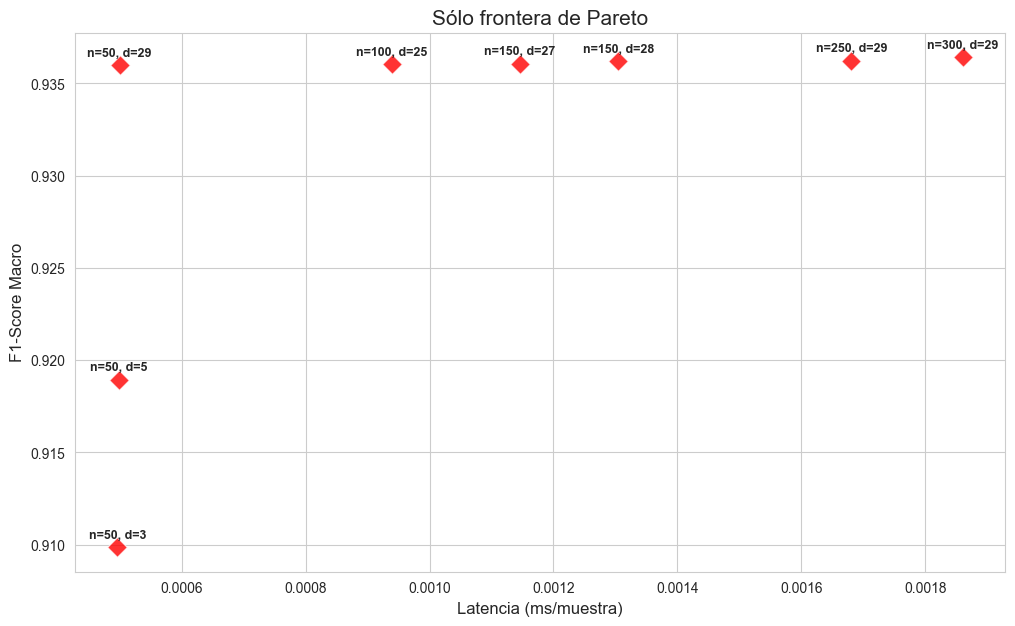
\includegraphics[width=0.8\textwidth]{../../images/PARETO_RF.png}
    \caption{Frontera de Pareto - Random Forest}
    \label{fig:pareto_rf}
\end{figure}

Se observa que configuraciones con un número reducido de árboles (n=50) y elevada profundidad (max_depth≈29) alcanzan valores de F1-macro prácticamente equivalentes a los modelos de mayor tamaño, pero con una latencia aproximadamente seis veces inferior. Este resultado evidencia que el incremento del número de árboles produce rendimientos decrecientes en términos de eficacia, mientras que el coste computacional continúa aumentando de forma significativa.

Hemos visto cómo reaccionan en test los modelos con los siguientes hiperparámetros elegidos:

1. (50, 29) Con solo 50 árboles alcanza un F1 casi idéntico al de modelos mucho más pesados
2. (100, 25) Es un punto intermedio, duplica los árboles respecto al anterior, pero gana robustez
3. (300, 28) Es más lento que los 3, pero es el que más F1 tiene

Los resultados son los siguientes:

\begin{table}[h]
    \centering
    \begin{tabular}{|l|c|c|c|c|c|}
        \hline
        \textbf{Perfil} & \textbf{n\_estimators} & \textbf{max\_depth} & \textbf{F1\_Test} & \textbf{Accuracy\_Test} & \textbf{Latencia (ms)} \\
        \hline
        Alta Eficiencia & 50 & 29 & 0.8731 & 0.8774 & 0.0012 \\
        \hline
        Equilibrado & 100 & 25 & 0.8809 & 0.8845 & 0.0018 \\
        \hline
        Máxima Precisión & 300 & 28 & 0.8766 & 0.8807 & 0.0055 \\
        \hline
    \end{tabular}
    \caption{Comparativa final de modelos Random Forest en el set de test}
    \label{tab:rf_comparison}
\end{table}